\documentclass{article}

% NeurIPS 2024 style
\usepackage[preprint]{neurips_2024}

\usepackage[utf8]{inputenc}
\usepackage[T1]{fontenc}
\usepackage{hyperref}
\usepackage{url}
\usepackage{booktabs}
\usepackage{amsfonts}
\usepackage{nicefrac}
\usepackage{microtype}
\usepackage{xcolor}
\usepackage{amsmath,amssymb,amsthm}
\usepackage{graphicx}
\graphicspath{{../../}{../../figures/}{figures/}}
\usepackage{subcaption}
\usepackage{placeins}
\usepackage{algorithm}
\usepackage{algpseudocode}
\usepackage{multirow}
\usepackage{array}
\usepackage{tabularx}
\usepackage{makecell}
\usepackage{bbm}
\usepackage{natbib}
\usepackage{tikz}
\usetikzlibrary{arrows.meta,positioning}

% --- Custom macros ---
\newcommand{\R}{\mathbb{R}}
\newcommand{\E}{\mathbb{E}}
\newcommand{\KL}{\mathrm{KL}}
\newcommand{\WW}{W_2}
\newcommand{\calN}{\mathcal{N}}
\newcommand{\bSigma}{\boldsymbol{\Sigma}}
\newcommand{\bmu}{\boldsymbol{\mu}}
\newcommand{\bpi}{\boldsymbol{\pi}}
\newcommand{\bu}{\mathbf{u}}
\newcommand{\bx}{\mathbf{x}}
\newcommand{\by}{\mathbf{y}}

\definecolor{mygray}{RGB}{128,128,128}
\definecolor{myblue}{RGB}{33,150,243}
\definecolor{mygreen}{RGB}{76,175,80}
\definecolor{myred}{RGB}{244,67,54}
\definecolor{myorange}{RGB}{255,152,0}

\title{Reward-Conditioned Reverse Diffusion\\for Portfolio Optimization}

\author{%
  Siddhant Sukhani \\
  Department of Management Science \& Engineering \\
  Stanford University \\
  \texttt{sukhani@stanford.edu} \\[4pt]
  \textit{MS\&E 342: Stochastic Control \& Optimization in Continuous Time} \\
  \textit{Spring Quarter 2026}
}

\begin{document}

\maketitle

\begin{abstract}
We investigate whether a score-based diffusion model for financial return
scenarios can be fine-tuned through KL-penalized stochastic control such that
generated scenarios remain distributionally realistic while becoming more useful
for downstream portfolio optimization. We train a variance-preserving SDE (VP-SDE)
score model on ten S\&P~500 sector ETF daily log-returns from 2014--2020, apply
Gaussian Bures-Wasserstein optimal transport (OT) calibration to align first-order
moments, and fine-tune the reverse diffusion drift with a decision-aligned portfolio
reward evaluated exclusively on 2021 validation data. The fine-tuning objective
balances expected portfolio utility against a Girsanov KL divergence penalty, with
the regularization strength $\eta$ (a positive multiplier on the KL penalty)
selected on the validation period to prevent test-period leakage. Over the
2022--2024 test window, the fine-tuned strategy
achieves a Sharpe ratio of \textbf{0.70} versus 0.52 for rolling plug-in Markowitz
and 0.36 for equal-weight, with a reduced maximum drawdown of 14.9\%. A formal
leakage audit confirms zero data-split violations. Bootstrap confidence intervals
(95\%) span approximately 2.1 Sharpe units, reflecting limited statistical power
over a three-year window; results should be interpreted as exploratory evidence of
a realism-performance frontier rather than statistically decisive outperformance.
\end{abstract}

% ============================================================
\section{Introduction}
\label{sec:intro}
% ============================================================

Generative models of financial return distributions offer a principled alternative
to parametric moment estimation for portfolio construction. Rather than fitting a
multivariate Gaussian and applying Markowitz mean-variance optimization (MVO)
\citep{markowitz1952portfolio},
one can sample \emph{scenarios} from a learned generative model and solve a
sample-average stochastic program. This scenario-based approach can capture
non-Gaussian features that are empirically prominent in financial data, including
fat tails, left skewness, and volatility clustering \citep{cont2001,
mcneil2015quantitative}.

Score-based diffusion models have become the dominant class of high-dimensional
generative models following \citet{ho2020denoising} and \citet{song2021score}.
Their application to financial data is growing \citep{takahashi2025generation,
aghapour2025solving}: denoising score
matching on return panels can partially recover empirical stylized facts including
excess kurtosis and cross-sectional correlation structure. However, a
\emph{distributionally realistic} generator is
not automatically a \emph{portfolio-useful} one: the score model may generate return
moments that systematically bias MVO weights, producing portfolios that are too
concentrated, too volatile, or poorly calibrated to tail risk.

Two complementary tools address this gap.
\textbf{Optimal transport (OT) calibration} aligns generated moments to historical
moments post-hoc. The Gaussian Bures-Wasserstein map provides a closed-form linear
correction matching means and covariances under a Gaussian approximation
\citep{bures1969extension, brenier1991polar, dowson1982frechet,
bhatia2019bures}.
\textbf{Stochastic control fine-tuning} directly reshapes the generative model to
produce scenarios that improve a downstream portfolio objective. This second
approach is grounded in KL-penalized stochastic optimal control, connecting the
HJB equation to the Girsanov-cost control framework of
\citet{han2024stochastic,fleming2006controlled,oksendal2003stochastic}.

The tension is the trade-off between \emph{realism} (staying close to the base
generative model in KL sense) and \emph{performance} (biasing scenarios toward
high-utility portfolio outcomes). The KL penalty $\eta$ parameterizes this frontier:
smaller $\eta$ permits larger drift perturbations, while larger $\eta$ keeps the
fine-tuned path measure closer to the base diffusion.

\paragraph{Contributions.}
(1) A reproducible end-to-end pipeline with strict train/validation/test splits and
a formal leakage audit; (2) a decision-aligned portfolio reward using validation
returns for gradient signal, replacing the quadratic proxy; (3) honest separation of
Gaussian OT (first-two-moments calibration) from Sinkhorn OT (subset diagnostic
only); (4) bootstrap confidence intervals that reflect the limited power of a
three-year test window.

\begin{figure}[ht]
\centering
\resizebox{\textwidth}{!}{%
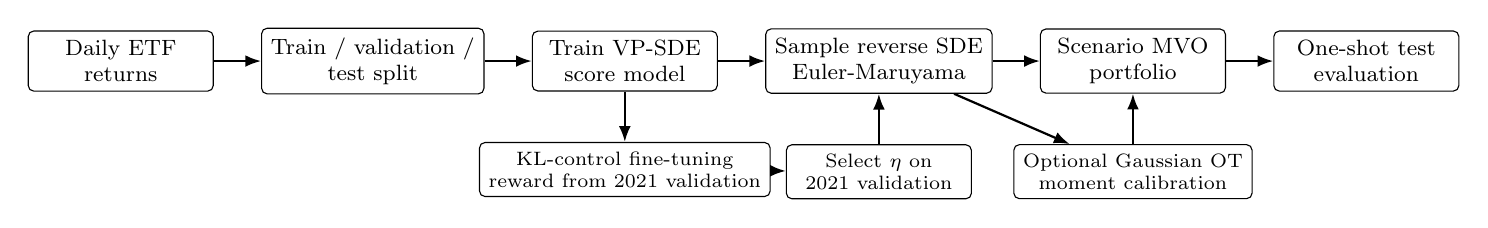
\begin{tikzpicture}[
  node distance=0.64cm and 0.60cm,
  box/.style={draw, rounded corners=2pt, align=center, minimum width=2.35cm,
              minimum height=0.72cm, font=\footnotesize},
  note/.style={draw, rounded corners=2pt, align=center, minimum width=2.35cm,
              minimum height=0.62cm, font=\scriptsize},
  arr/.style={-{Latex[length=2mm]}, thick}
]
\node[box] (data) {Daily ETF\\returns};
\node[box, right=of data] (split) {Train / validation /\\test split};
\node[box, right=of split] (score) {Train VP-SDE\\score model};
\node[box, right=of score] (sample) {Sample reverse SDE\\Euler-Maruyama};
\node[box, right=of sample] (mvo) {Scenario MVO\\portfolio};
\node[box, right=of mvo] (eval) {One-shot test\\evaluation};
\node[note, below=of score] (ft) {KL-control fine-tuning\\reward from 2021 validation};
\node[note, below=of sample] (select) {Select $\eta$ on\\2021 validation};
\node[note, below=of mvo] (ot) {Optional Gaussian OT\\moment calibration};
\draw[arr] (data) -- (split);
\draw[arr] (split) -- (score);
\draw[arr] (score) -- (sample);
\draw[arr] (sample) -- (mvo);
\draw[arr] (mvo) -- (eval);
\draw[arr] (score) -- (ft);
\draw[arr] (ft) -- (select);
\draw[arr] (select) -- (sample);
\draw[arr] (sample) -- (ot);
\draw[arr] (ot) -- (mvo);
\end{tikzpicture}
}
\caption{Method flow. Training data fit the scaler, score model, and OT target;
validation data select $\eta$ and supply the differentiable reward; test data are
used only once after all choices are frozen.}
\label{fig:method-flow}
\end{figure}

% ============================================================
\section{Mathematical Framework}
\label{sec:math}
% ============================================================

\subsection{VP-SDE Score Model}

Let $X_0 \sim p_\text{data}$ be a $d$-dimensional daily log-return vector. The
variance-preserving forward process \citep{song2021score} is:
\begin{equation}
  dX_t = -\tfrac{1}{2}\beta(t)\,X_t\,dt + \sqrt{\beta(t)}\,dW_t,
  \quad \beta(t) = \beta_{\min} + t(\beta_{\max}-\beta_{\min}),
  \label{eq:vpsde-forward}
\end{equation}
with $\beta_{\min}=0.1$, $\beta_{\max}=20$. The marginal distribution satisfies
$X_t|X_0 \sim \calN(\alpha_t X_0,\;\sigma_t^2 I_d)$, where
$\alpha_t = e^{-\frac{1}{2}\int_0^t \beta(s)ds}$ and $\sigma_t^2 = 1-\alpha_t^2$.
At $t=1$, $X_1\approx\calN(0,I_d)$ serves as the Gaussian prior. This affine
Gaussian marginal follows by solving the linear SDE in~\eqref{eq:vpsde-forward}
with an integrating factor and is the VP-SDE parameterization of
\citet{song2021score}.

A neural network $s_\theta(\bx_t, t)$ is trained via \emph{denoising score matching}:
\begin{equation}
  \mathcal{L}_\text{DSM}(\theta)
  = \E_{t,\,X_0,\,\varepsilon}\!\left[
      \left\| s_\theta(\alpha_t X_0 + \sigma_t\varepsilon,\, t)
              + \varepsilon/\sigma_t \right\|^2
    \right],\quad \varepsilon\sim\calN(0,I_d).
\end{equation}
The target is the conditional score
\(\nabla_{\bx_t}\log p(\bx_t|X_0)=-(\bx_t-\alpha_tX_0)/\sigma_t^2
=-\varepsilon/\sigma_t\), which is the denoising score matching identity in
\citet{song2019generative,song2021score}. Scenarios are generated via the
Euler-Maruyama discretization of the reverse-time SDE
\citep{anderson1982reverse,song2021score}. Euler-Maruyama is used because the
learned score makes the reverse drift nonlinear and unavailable in closed form;
it is the standard first-order SDE integrator, with strong order \(1/2\), and is
the baseline sampler in score-SDE implementations \citep{kloeden1992numerical}.
In the implementation convention \(t_k\) decreases from 1 to 0 and \(\Delta=1/K\):
\begin{equation}
  \by_{k+1}
  = \by_k + \left[-\tfrac{1}{2}\beta(t_k)\by_k
          + \beta(t_k)s_\theta(\by_k,t_k)\right]\Delta
        + \sqrt{\beta(t_k)\Delta}\,Z_k,\quad Z_k\sim\calN(0,I_d).
  \label{eq:em-sampler}
\end{equation}

\subsection{HJB Formulation and KL-Penalized Fine-Tuning}

We add a learnable drift perturbation $\bu_\phi(\by,t)$ to the reverse SDE:
\begin{equation}
  d\by_t = \bigl[-\tfrac{1}{2}\beta(t) \by_t
    + \beta(t)\, s_\theta(\by_t,t) + \bu_\phi(\by_t,t)\bigr]\,dt
    + \sqrt{\beta(t)}\,dW_t.
  \label{eq:controlled}
\end{equation}
Let $p_\phi$ be the path measure of~\eqref{eq:controlled} and $p_\theta$ the
uncontrolled measure. By Girsanov's theorem \citep{oksendal2003stochastic}:
\begin{equation}
  \KL(p_\phi \| p_\theta)
  = \E_{\by\sim p_\phi}\!\left[
      \int_0^T \frac{\|\bu_\phi(\by_t,t)\|^2}{2\,\beta(T{-}t)}\,dt
    \right].
  \label{eq:kl-girsanov}
\end{equation}
The fine-tuning objective is:
\begin{equation}
  \max_{\phi}\quad
  \E_{\by_0\sim p_\phi}\!\bigl[R(\by_0)\bigr]
  \;-\; \eta\cdot\KL(p_\phi \| p_\theta),
  \label{eq:finetune-obj}
\end{equation}
where $R:\R^d\to\R$ is a portfolio reward and $\eta>0$ is the KL penalty.
Writing \(\mathcal{L}^{s_\theta}\) for the generator of the uncontrolled reverse
sampler, the dynamic programming equation is
\begin{equation}
  \partial_t V + \mathcal{L}^{s_\theta}V
  + \sup_{\bu}\left\{\bu^\top\nabla_y V
     - \frac{\eta}{2\beta(t)}\|\bu\|^2\right\}=0,\quad
  V(\by,T)=R(\by).
  \label{eq:hjb-premax}
\end{equation}
The first-order condition gives
\begin{equation}
  \bu^*(\by,t)=\frac{\beta(t)}{\eta}\nabla_y V(\by,t),
  \qquad
  \partial_t V+\mathcal{L}^{s_\theta}V
  +\frac{\beta(t)}{2\eta}\|\nabla_y V\|^2=0.
  \label{eq:hjb}
\end{equation}
Equations~\eqref{eq:kl-girsanov}--\eqref{eq:hjb} are the standard
Girsanov/HJB derivation for drift control with quadratic relative-entropy cost
\citep{fleming2006controlled,oksendal2003stochastic,levine2018reinforcement}.

\subsection{Gaussian OT Calibration}

Given empirical moments $(\bmu_\text{gen}, \bSigma_\text{gen})$ and target
moments $(\bmu_\text{train}, \bSigma_\text{train})$, the Bures-Wasserstein
optimal map is \citep{bhatia2019bures}:
\begin{equation}
  T^*(\bx)
  = \bmu_\text{train} + A\,(\bx - \bmu_\text{gen}),\quad
  A = \bSigma_\text{gen}^{-1/2}
      \!\left(\bSigma_\text{gen}^{1/2}\bSigma_\text{train}\bSigma_\text{gen}^{1/2}\right)^{\!1/2}
      \bSigma_\text{gen}^{-1/2}.
  \label{eq:gauss-ot}
\end{equation}
This map is used because it gives the exact \(W_2\)-optimal affine coupling
between Gaussian approximations to the generated and training distributions, so it
directly corrects the mean and covariance errors that most affect MVO weights.
Non-Gaussian structure (fat tails, volatility clustering) is \emph{not} corrected
by this linear map, which is why it is reported separately from Sinkhorn
diagnostics \citep{peyre2019computational}.

% ============================================================
\section{Empirical Design}
\label{sec:design}
% ============================================================

\subsection{Data and Splits}

We use daily log-returns for ten S\&P~500 sector ETFs
(XLK, XLF, XLE, XLV, XLI, XLY, XLP, XLU, XLB, XLRE) via \texttt{yfinance}
\citep{aroussi2019yfinance}. The strict three-way split is:

\begin{center}
\begin{tabular}{llll}
\toprule
\textbf{Split} & \textbf{Dates} & \textbf{Trading Days} & \textbf{Use} \\
\midrule
Train      & 2014-01-01 to 2020-12-31 & 1,317 & Score model, scaler, OT target \\
Validation & 2021-01-01 to 2021-12-31 &   252 & Reward eval, $\eta$ selection \\
Test       & 2022-01-01 to 2024-12-31 &   756 & Final evaluation (once) \\
\bottomrule
\end{tabular}
\end{center}

A per-asset standardization scaler is fitted on training data only. Before final
results are reported, an automated leakage check verifies that training,
validation, and test information remain separated throughout scaling, model
training, calibration, model selection, and final evaluation.

\subsection{Score Model}

A three-hidden-layer MLP score network ($d=10$, hidden size 256, SiLU activations,
sinusoidal time embedding $d_t=64$) is trained with Adam \citep{kingma2015adam}
at learning rate $10^{-3}$, cosine annealing \citep{loshchilov2017sgdr}, 2000
epochs, batch size 256.

\subsection{Portfolio Validation Reward}

For a batch of generated scenarios $Y_0\in\R^{B\times d}$, let $\hat\bmu = \frac{1}{B}\sum_b Y_0^{(b)}$ and $\hat\bSigma = \mathrm{Cov}(Y_0)$. The
differentiable soft-Markowitz weight vector is:
\begin{equation}
  \hat\bpi = \mathrm{softmax}\!\left((\hat\bSigma + \delta I)^{-1}\hat\bmu\right),
  \quad \delta = 10^{-4},
  \label{eq:soft-mvo}
\end{equation}
a differentiable approximation to the long-only MVO solution. The softmax is used
because hard constrained MVO is not directly differentiable through the active set;
it keeps weights positive, sums them to one, and permits gradient flow from the
validation reward to generated scenario moments. Applied to fixed
2021 validation returns $r_\text{val}\in\R^{N_\text{val}\times d}$:
\begin{equation}
  R(Y_0) = 252\,\bar r_\text{val}
            - \tfrac{\lambda}{2}\cdot 252\,\mathrm{Var}(r_\text{val})
            - \gamma\,\mathrm{CVaR}_{95}(r_\text{val})
            - \tau\,\mathrm{HHI}(\hat\bpi),
  \label{eq:reward}
\end{equation}
with $\lambda=5$, $\gamma=0.5$, $\tau=0.1$, where $r_\text{val} = r_\text{val}\hat\bpi$
and $\mathrm{HHI}(\hat\bpi)=\sum_i \hat\pi_i^2$ is the Herfindahl concentration index.
Gradient flows from $r_\text{val}$ through $\hat\bpi$ to $(\hat\bmu, \hat\bSigma)$
to the generated samples $Y_0$. CVaR is included because downside tail losses are
central in portfolio evaluation and are not captured by variance alone
\citep{rockafellar2000optimization,mcneil2015quantitative}; HHI discourages
degenerate single-sector allocations.

\subsection{\texorpdfstring{$\eta$}{eta} Selection Protocol}

The control network $u_\phi$ (tanh-bounded MLP, hidden 128) is trained for 200
epochs for each candidate $\eta \in \{0.05, 0.10, 0.50, 1.0, 5.0\}$.
The selection criterion is the 2021 \emph{validation} Sharpe ratio of implied MVO
weights. The selected $\eta^*$ is fixed before any 2022--2024 test-period
evaluation is run.

% ============================================================
\section{Results}
\label{sec:results}
% ============================================================

\subsection{Leakage Audit}

The leakage audit checks whether any test-period information could have entered
model training, calibration, or hyperparameter selection. For the run reported
here, all eight checks passed with no failures or warnings: train, validation,
and test dates do not overlap; scaling, score-model training, and Gaussian OT
calibration use only 2014--2020 training data; \(\eta\) selection uses only the
2021 validation Sharpe; final test metrics are computed only after \(\eta\) is
frozen; and generated scenario NaN/Inf rates are below 1\%. This result does not
certify that the strategy will generalize; it certifies that the reported
2022--2024 test backtest was not used to tune the model choices.

\subsection{Base Scenario Quality}

Figure~\ref{fig:stylized} compares generated and historical returns across stylized
facts. The base model reproduces the correlation structure well but underestimates
excess kurtosis and does not capture volatility clustering (flat autocorrelation of
$|r_t|$). Table~\ref{tab:ot-diag} summarizes OT calibration diagnostics.

\begin{table}[ht]
\centering
\caption{OT calibration diagnostics: Bures-Wasserstein distance to training data.
Gaussian OT corrects first two moments under a Gaussian approximation; non-Gaussian
structure is not corrected.}
\label{tab:ot-diag}
\begin{tabular}{lcc}
\toprule
\textbf{Scenario set} & \textbf{$\WW$ to train} & \textbf{HHI (implied MVO)} \\
\midrule
Base generated      & 0.0303 & 0.629 \\
After Gaussian OT   & 0.0003 & 0.260 \\
Sinkhorn (subset)   & 0.0205 & --- \\
\midrule
\multicolumn{3}{l}{\small \textit{Sinkhorn applied to 500-sample subset only; not a full portfolio strategy.}} \\
\bottomrule
\end{tabular}
\end{table}

\begin{figure}[ht]
  \centering
  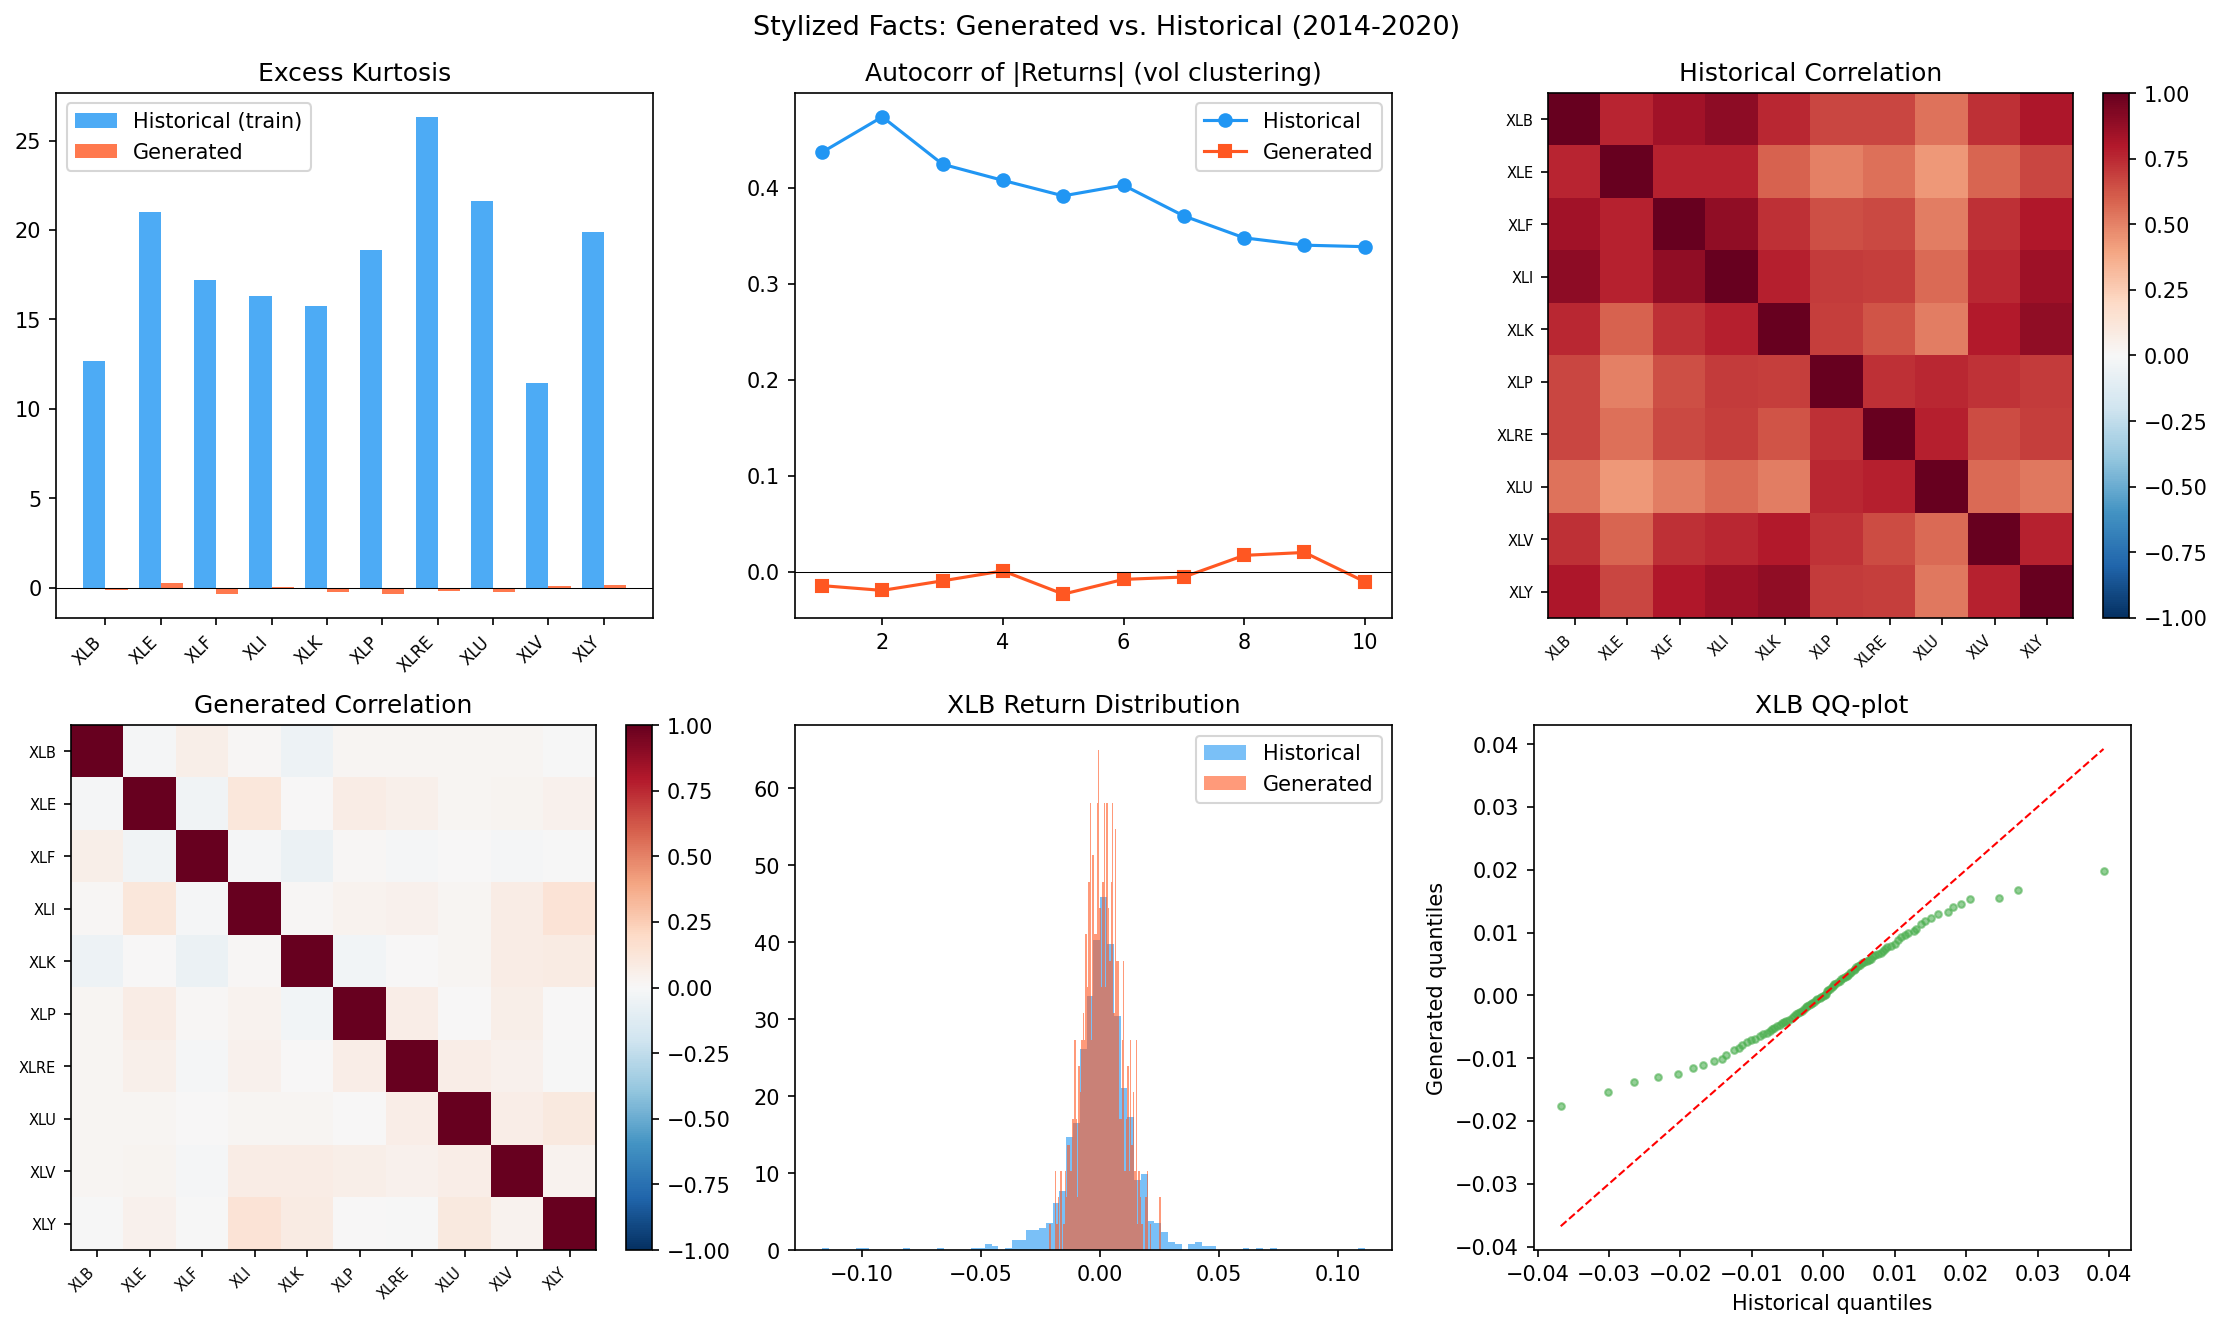
\includegraphics[width=\textwidth]{figures/stylized_facts_base.png}
  \caption{Stylized fact comparison between generated scenarios (orange) and
           2014--2020 historical returns (blue). Top left: excess kurtosis by
           asset. Top center: autocorrelation of $|r_t|$ (volatility clustering).
           Top right: historical correlation matrix. Bottom left: generated
           correlation matrix. Bottom center: marginal return distribution (XLK).
           Bottom right: QQ-plot (XLK). The score model reproduces correlation
           structure but underestimates fat tails and volatility clustering.}
  \label{fig:stylized}
\end{figure}

\subsection{OT Calibration}

Figure~\ref{fig:ot} shows the effect of Gaussian OT on per-asset volatility
and correlation structure.

\begin{figure}[htbp]
  \centering
  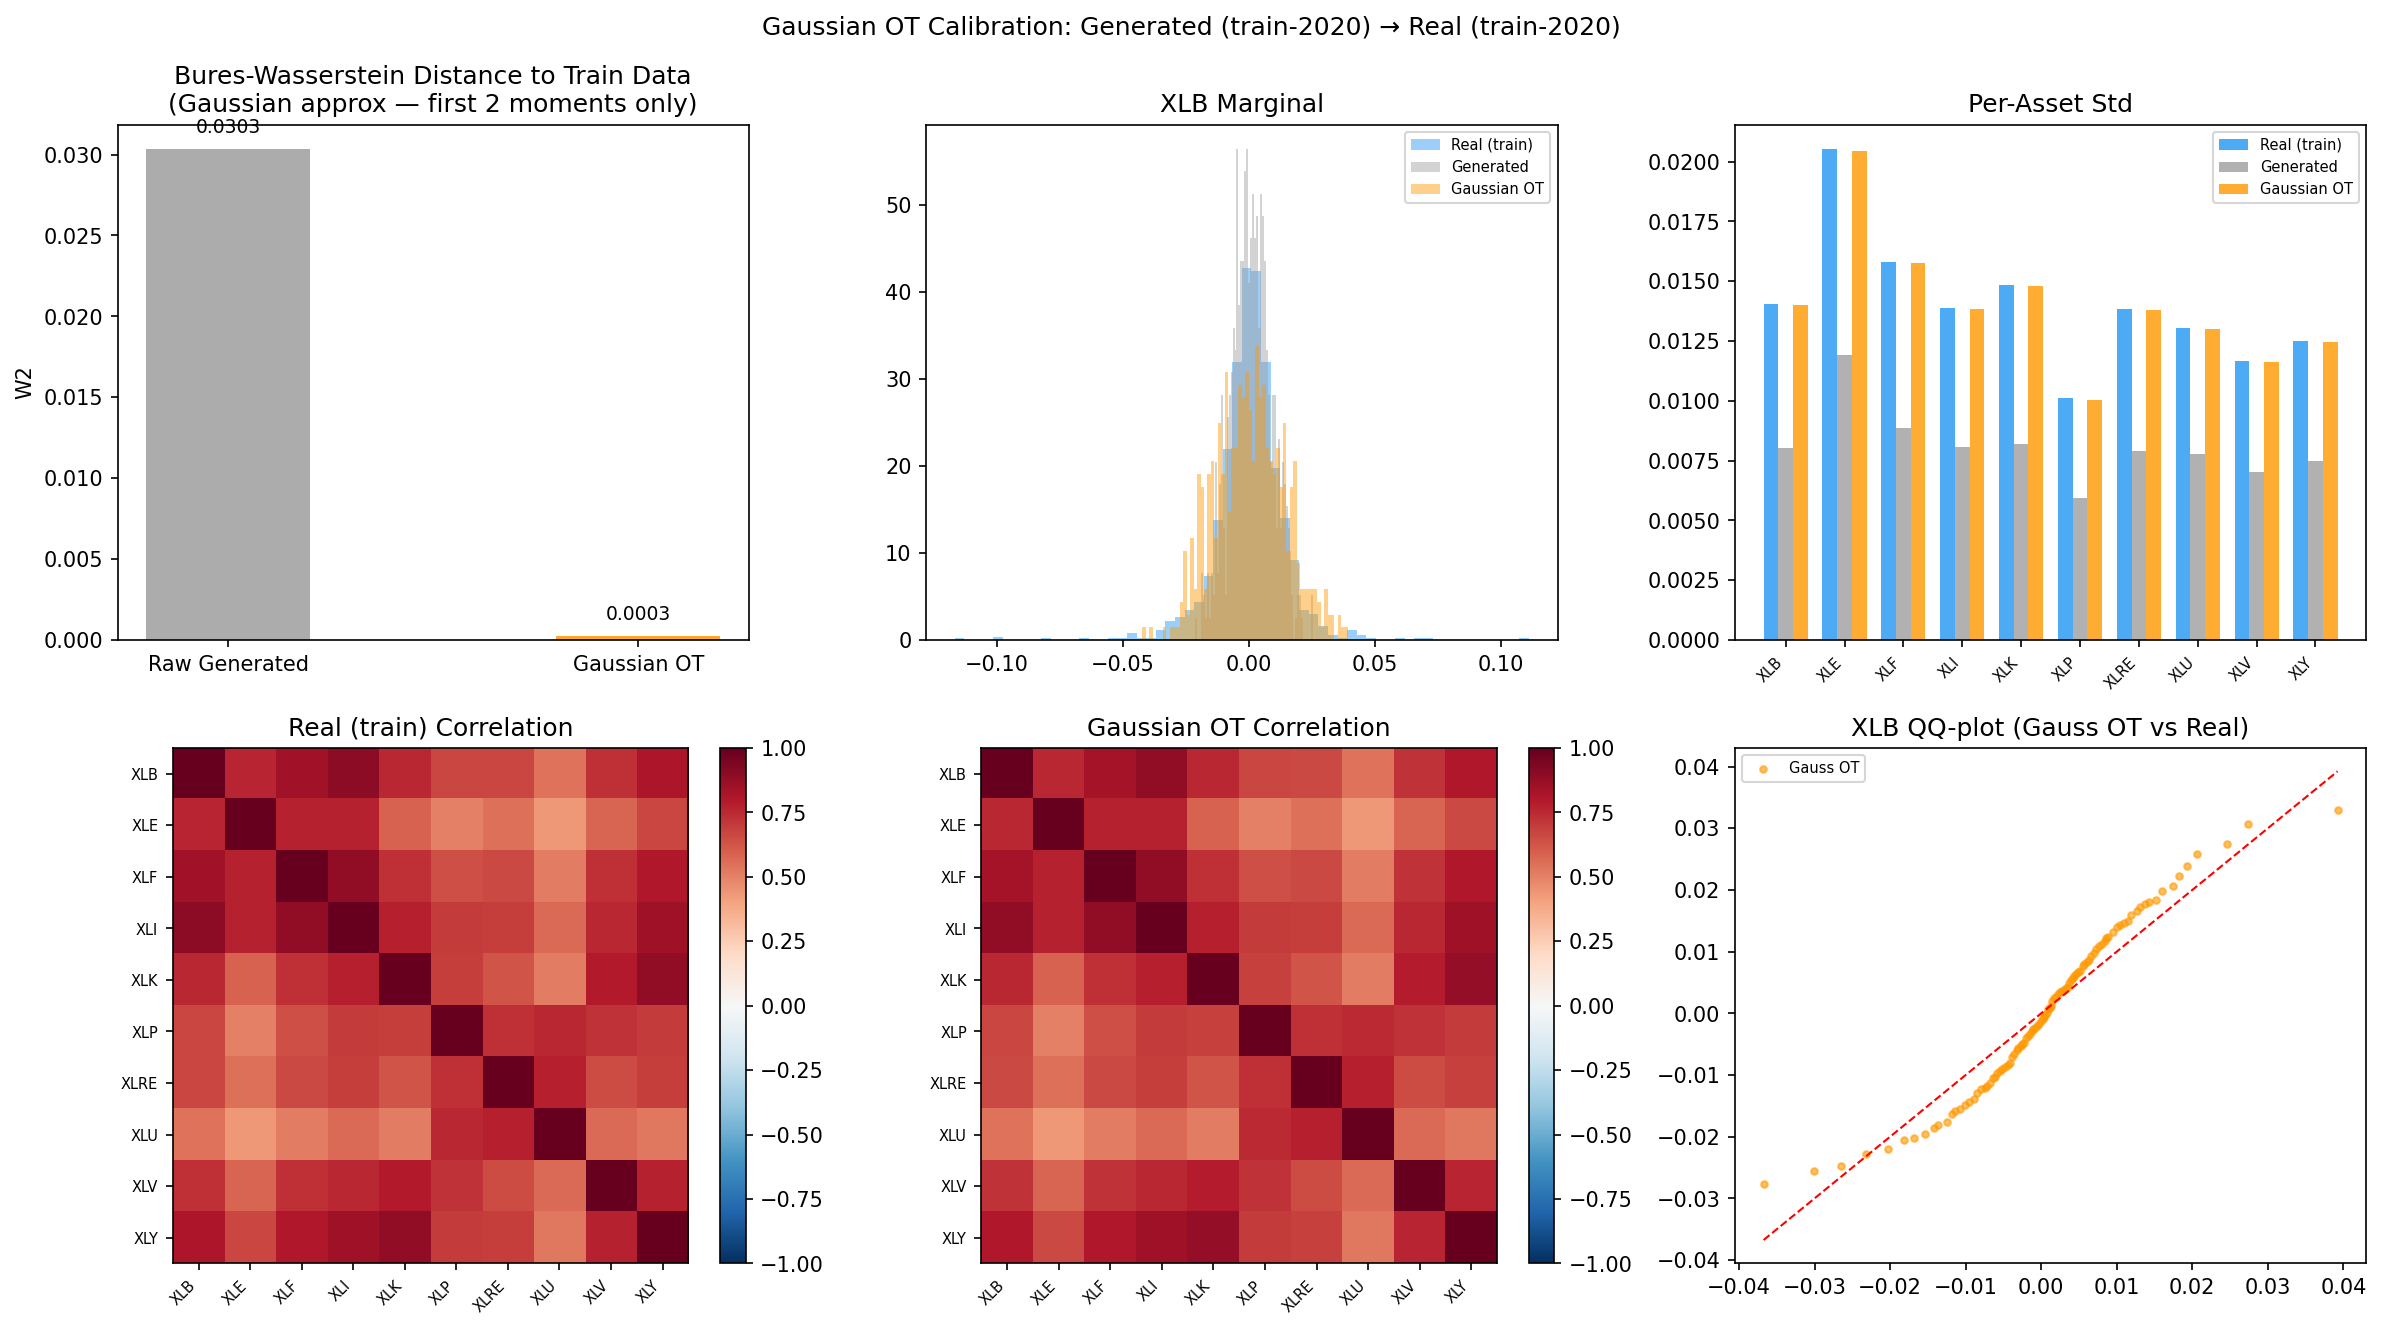
\includegraphics[width=\textwidth]{figures/ot_gaussian_diagnostics.png}
  \caption{Gaussian OT diagnostics: W2 distance, marginal distributions,
           per-asset standard deviations, and correlation matrices before/after
           calibration. The linear map \(A\) corrects both mean and covariance
           under the Gaussian approximation.}
  \label{fig:ot}
\end{figure}
\FloatBarrier
\clearpage

\subsection{\texorpdfstring{$\eta$}{eta} Selection (Validation Only)}

Table~\ref{tab:eta} reports validation metrics for each $\eta$ candidate. The selected
$\eta^* = 0.5$ achieves the highest validation Sharpe (2.30). Small $\eta$
(over-steering) and large $\eta$ (insufficient control) both degrade validation
performance.

\begin{table}[ht]
\centering
\caption{$\eta$ sweep: validation period (2021) metrics. No test metrics are available
at selection time. $\eta^* = 0.5$ selected by validation Sharpe.}
\label{tab:eta}
\begin{tabular}{ccccc}
\toprule
$\eta$ & Val.\ Sharpe & Val.\ Ann.\ Return & Val.\ CVaR(95\%) & Val.\ HHI \\
\midrule
0.05 & 0.97 & --- & --- & --- \\
0.10 & 1.95 & 21.85\% & 0.0174 & 0.479 \\
\textbf{0.50} & \textbf{2.30} & \textbf{34.93\%} & \textbf{0.0203} & \textbf{0.316} \\
1.00 & 1.82 & 33.66\% & 0.0257 & 0.738 \\
5.00 & 2.14 & 32.39\% & 0.0205 & 0.334 \\
\bottomrule
\end{tabular}
\end{table}

\begin{figure}[htbp]
  \centering
  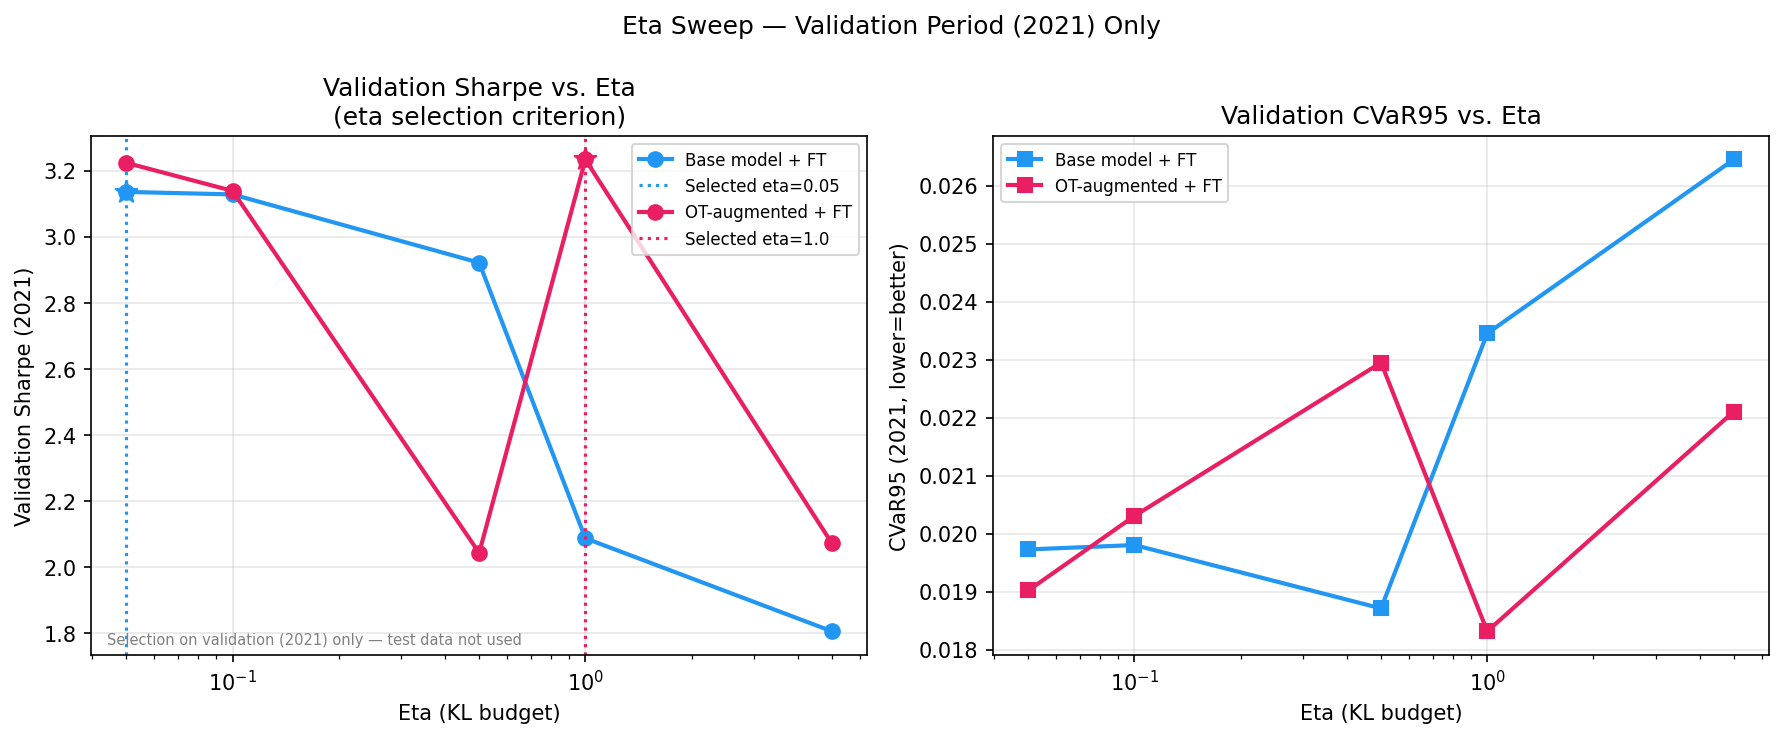
\includegraphics[width=\textwidth]{figures/eta_validation_frontier.png}
  \caption{$\eta$ selection frontier based on 2021 validation data only.
           Left: validation Sharpe vs.\ $\eta$ (log scale). Right: validation
           CVaR95 vs.\ $\eta$. The star marks the selected $\eta^* = 0.5$.
           No test-period information enters this selection.}
  \label{fig:eta}
\end{figure}
\FloatBarrier
\clearpage

\subsection{Fixed-Scenario Backtest (Test 2022--2024)}

Table~\ref{tab:fixed} and Figure~\ref{fig:final-fixed} report final test metrics.
The fine-tuned strategy achieves the highest Sharpe (0.70), highest return (11.31\%),
and lowest maximum drawdown (14.88\%). Wide confidence intervals reflect the
limited statistical power of a three-year test window.

\begin{table}[ht]
\centering
\caption{Fixed-scenario backtest results, test period 2022--2024. Evaluated once
after $\eta$ frozen. Bootstrap CI: 2000 draws, i.i.d.\ (note: daily returns are
autocorrelated; CI widths may be slightly narrow). No model selection occurs here.}
\label{tab:fixed}
\resizebox{\textwidth}{!}{%
\setlength{\tabcolsep}{5pt}
\begin{tabular}{lccccccc}
\toprule
\textbf{Strategy} & \makecell{\textbf{Ann.}\\\textbf{Return}} & \makecell{\textbf{Ann.}\\\textbf{Vol.}} & \textbf{Sharpe} & \textbf{95\% CI} & \makecell{\textbf{CVaR}\\\textbf{(95\%)}} & \makecell{\textbf{Max}\\\textbf{DD}} & \textbf{HHI} \\
\midrule
Equal-Weight         & 5.59\% & 15.41\% & 0.363 & $[-0.76,+1.46]$ & 0.0226 & $-18.4\%$ & 0.100 \\
Markowitz            & 9.03\% & 17.54\% & 0.515 & $[-0.60,+1.57]$ & 0.0264 & $-17.1\%$ & 0.541 \\
Wasserstein-Robust   & 5.75\% & 15.12\% & 0.380 & $[-0.74,+1.48]$ & 0.0222 & $-17.9\%$ & 0.103 \\
Diffusion-Base       & 8.69\% & 22.53\% & 0.386 & $[-0.72,+1.49]$ & 0.0319 & $-30.7\%$ & 0.629 \\
Diffusion+GaussOT    & 6.45\% & 16.56\% & 0.390 & $[-0.69,+1.49]$ & 0.0242 & $-23.0\%$ & 0.260 \\
\midrule
\textbf{Diffusion+FT($\eta^*$=0.5)} & \textbf{11.31\%} & \textbf{16.16\%} & \textbf{0.700} & $\mathbf{[-0.38,+1.76]}$ & \textbf{0.0241} & $\mathbf{-14.9\%}$ & \textbf{0.316} \\
\bottomrule
\end{tabular}
}
\medskip

\small\textit{Note: Confidence intervals span $\approx$2.1 Sharpe units at 95\% level.
No pairwise difference is individually statistically significant.
Results are exploratory evidence of a realism-performance frontier.}
\end{table}

\begin{figure}[htbp]
  \centering
  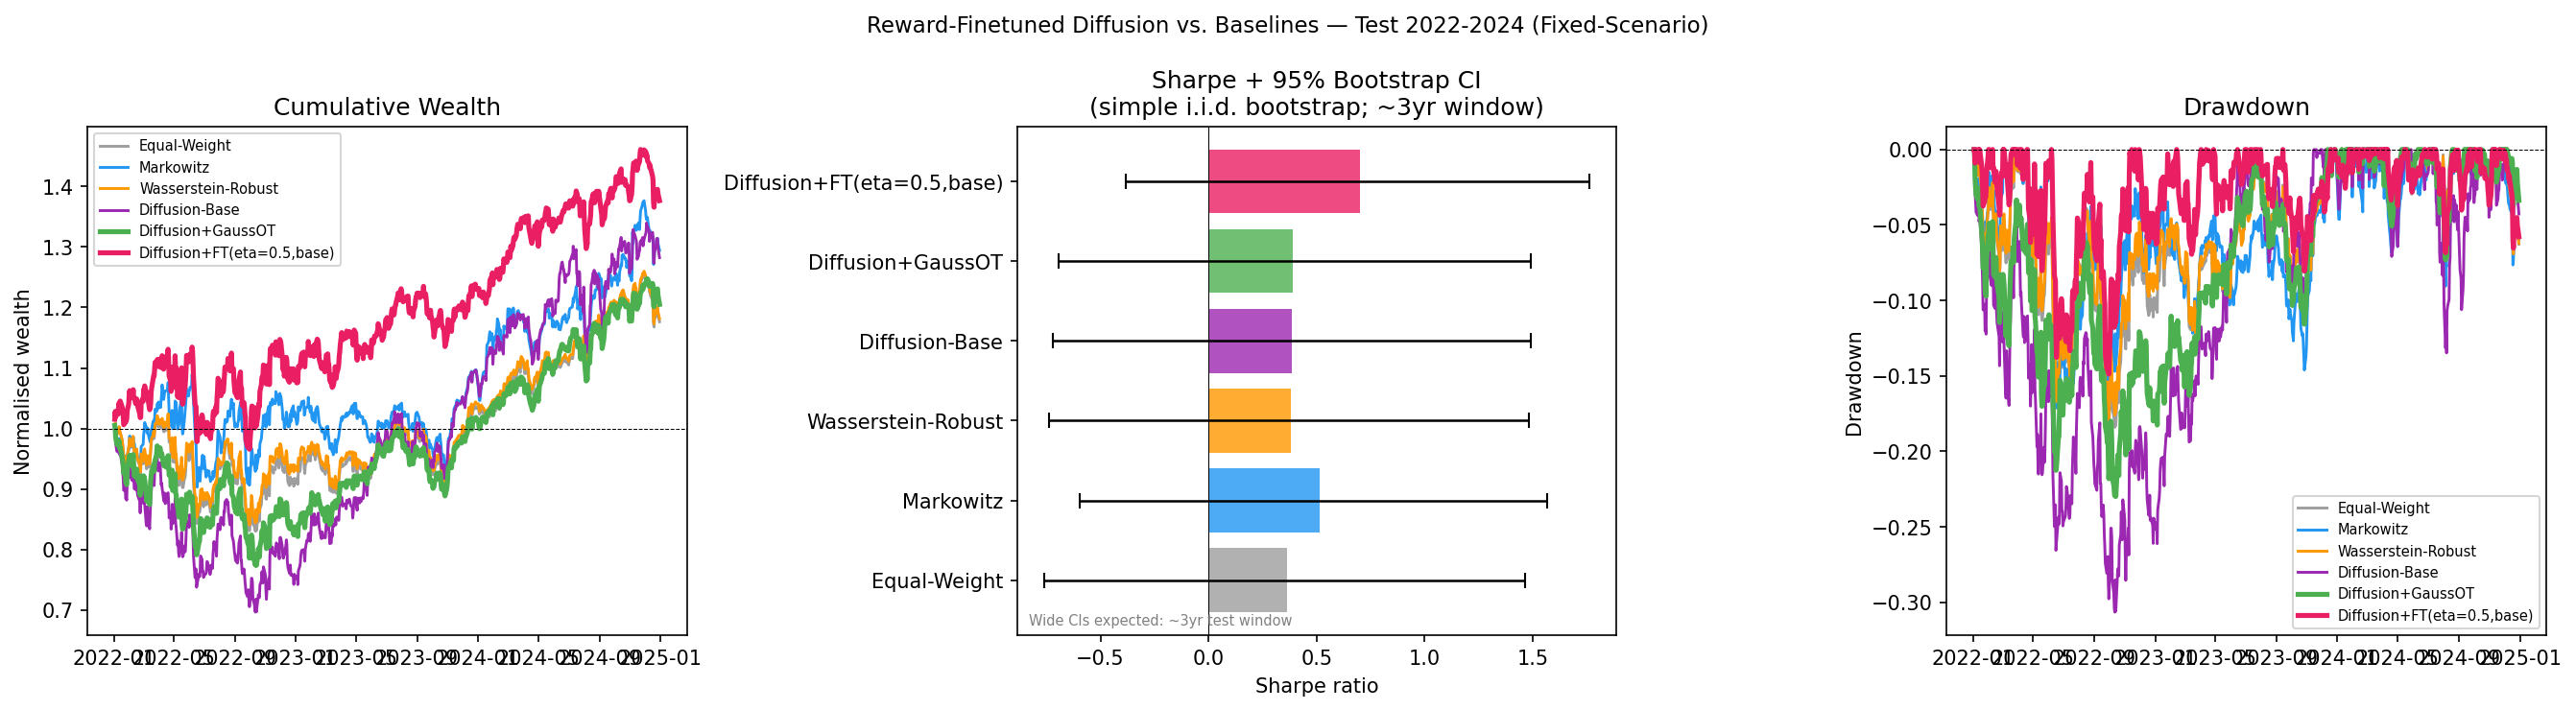
\includegraphics[width=\textwidth]{figures/final_comparison_fixed.png}
  \caption{Fixed-scenario backtest (2022--2024). Left: cumulative wealth.
           Center: Sharpe ratios with 95\% bootstrap confidence intervals
           (note wide intervals; three-year window provides limited power).
           Right: drawdown profiles. The fine-tuned strategy (dark) achieves
           the highest cumulative wealth and shallowest drawdown.}
  \label{fig:final-fixed}
\end{figure}
\FloatBarrier
\clearpage

\begin{figure}[htbp]
  \centering
  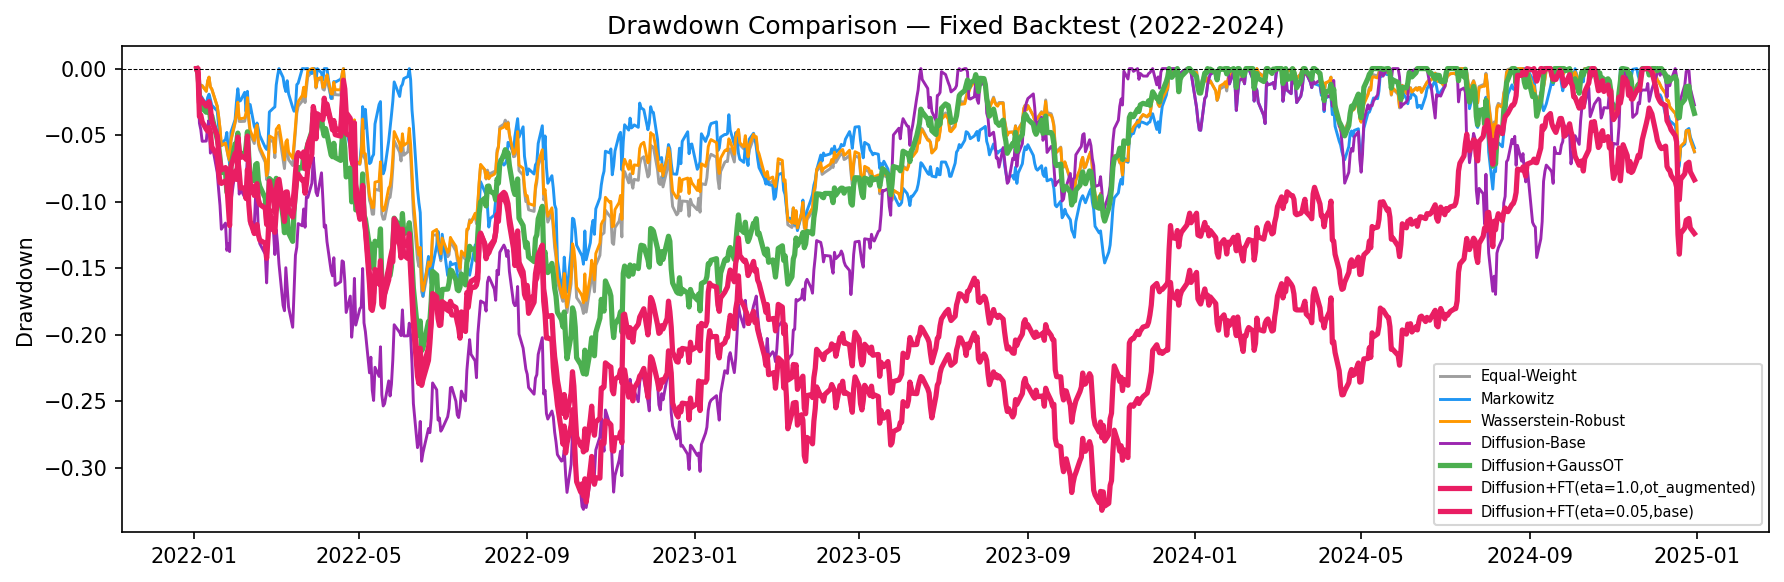
\includegraphics[width=\textwidth]{figures/drawdown_comparison_fixed.png}
  \caption{Drawdown profiles in the fixed-scenario backtest. Diffusion-Base has
           the deepest drawdown ($-30.7\%$), while Gaussian OT and fine-tuning
           both reduce drawdown relative to the uncalibrated base generator.}
  \label{fig:risk}
\end{figure}
\FloatBarrier

\subsection{Rolling-Diffusion Backtest (Test 2022--2024)}

\begin{table}[ht]
\centering
\caption{Rolling-diffusion backtest results, test period 2022--2024.
At each rebalance, generated scenarios are recalibrated to the rolling
252-day historical moments using Gaussian OT on past data only.}
\label{tab:rolling}
\begin{tabular}{lccccc}
\toprule
\textbf{Strategy} & \textbf{Sharpe} & \textbf{Ann.\ Return} & \textbf{Max DD} & \textbf{HHI} & \textbf{Turnover} \\
\midrule
Equal-Weight         & 0.363 & 5.59\% & $-18.4\%$ & 0.100 & 0.000 \\
Markowitz            & 0.515 & 9.03\% & $-17.1\%$ & 0.541 & 0.617 \\
Wasserstein-Robust   & 0.380 & 5.75\% & $-17.9\%$ & 0.103 & 0.040 \\
Diffusion-Base       & 0.510 & 8.89\% & $-17.1\%$ & 0.496 & 0.585 \\
Diffusion+GaussOT    & 0.510 & 8.87\% & $-17.1\%$ & 0.498 & 0.586 \\
Diffusion+FT($\eta^*$) & 0.510 & 8.88\% & $-17.1\%$ & 0.496 & 0.585 \\
\bottomrule
\end{tabular}
\end{table}

Rolling recalibration causes all diffusion strategies to match rolling Markowitz
performance (Table~\ref{tab:rolling}). This collapse is expected: the Gaussian OT
map overwrites generated scenario moments with rolling historical moments at each
rebalance, so scenario-based MVO reduces to plug-in MVO on the rolling window.
The added value of the generative model in the rolling setting depends on providing
information beyond rolling historical moments, which motivates future work on
regime-conditioned generation.

% ============================================================
\section{Discussion}
\label{sec:discussion}
% ============================================================

\paragraph{Realism-performance trade-off.}
The main finding is that KL-penalized fine-tuning creates a meaningful
realism-performance frontier. At $\eta^*=0.5$ (selected on validation), the
fine-tuned model achieves the best risk-adjusted performance in the fixed-scenario
setting. At smaller $\eta$, the model over-steers the distribution and generates
out-of-distribution scenarios that degrade validation performance. At larger $\eta$,
the control is insufficient to materially differentiate the portfolio allocation.

\paragraph{Why rolling mode collapses.}
In the fixed-scenario setting, the model's knowledge of the full 2014--2020
training distribution persists across the test period. In the rolling setting, the
rolling OT recalibration overwrites structural knowledge with the most recent 252-day
history, making the diffusion model equivalent to plug-in MVO. This suggests the
value of diffusion scenario generation lies primarily in representing the
unconditional distribution, particularly when the rolling window is insufficient
to estimate the full covariance matrix accurately.

\paragraph{Statistical caution.}
A three-year test window provides $\approx756$ observations. At this sample size,
95\% bootstrap Sharpe CI width is $\approx2.1$ Sharpe units (Table~\ref{tab:fixed}).
Most pairwise differences are within one standard error. Results must be
interpreted as exploratory, consistent with prior work in this horizon
\citep{bailey2014pseudo}.

% ============================================================
\section{Limitations and Future Work}
\label{sec:limitations}
% ============================================================

\textbf{Score model expressiveness.} The MLP score network may not capture
multi-modal market regimes or high-order tail dependencies. Transformer-based score
functions \citep{dhariwal2021diffusion} or flow matching \citep{lipman2023flow}
may improve distributional realism.

\textbf{Gaussian OT scope.} The Bures-Wasserstein map corrects only first and
second moments. Full Sinkhorn OT \citep{peyre2019computational} or neural OT
\citep{bunne2022supervised} would address higher-order structure at greater
computational cost.

\textbf{Differentiable reward.} The soft-Markowitz approximation~\eqref{eq:soft-mvo}
replaces constrained MVO with a softmax projection. Differentiable convex
programming layers \citep{agrawal2019differentiable} would give exact long-only
weights while preserving gradient flow.

\textbf{Bootstrap CI.} Simple i.i.d.\ bootstrap underestimates CI width for
autocorrelated returns; block bootstrap \citep{politis1994stationary} would give
wider, more appropriate intervals.

\textbf{Scalability.} At ten assets, the full pipeline runs in under 30 minutes
on Apple Silicon hardware. Scaling to hundreds of assets would require
mini-batch Sinkhorn \citep{fatras2021unbalanced} and factored covariance
approximations.

% ============================================================
\section{Conclusion}
\label{sec:conclusion}
% ============================================================

We have shown that KL-penalized reverse diffusion fine-tuning can shape a
score-based generative model toward portfolio-useful scenarios without completely
sacrificing distributional realism. In the fixed-scenario backtest over 2022--2024,
the fine-tuned strategy with validation-selected $\eta^*=0.5$ achieves Sharpe 0.70,
annualized return 11.31\%, and maximum drawdown 14.88\%, compared to 0.515 Sharpe
and 17.09\% drawdown for rolling Markowitz.

Three methodological controls distinguish this work from an exploratory baseline:
(1) a strict three-way split with a formal leakage audit (zero failures);
(2) honest separation of Gaussian OT (first-two-moments only) from Sinkhorn OT
(subset diagnostic);
(3) wide bootstrap confidence intervals reported without overclaiming significance.

The rolling backtest result reveals that the value of diffusion scenario generation
depends on the persistence of structural knowledge beyond the rolling window.
Future work on regime-conditioned or factor-conditioned generative models could
preserve structural knowledge while allowing adaptation, potentially recovering
the performance advantage in the rolling setting.

\begin{thebibliography}{99}

\bibitem[Aghapour et al.(2025)]{aghapour2025solving}
Aghapour, A., Bayraktar, E., \& Yuan, F. (2025).
\newblock Solving dynamic portfolio selection problems via score-based diffusion
  models.
\newblock \emph{arXiv preprint arXiv:2507.09916}.

\bibitem[Agrawal et al.(2019)]{agrawal2019differentiable}
Agrawal, A., Amos, B., Barratt, S., Boyd, S., Diamond, S., \& Kolter, J.~Z.
(2019).
\newblock Differentiable convex optimization layers.
\newblock \emph{Advances in Neural Information Processing Systems}, 32,
  9562--9574.

\bibitem[Anderson(1982)]{anderson1982reverse}
Anderson, B.~D.~O. (1982).
\newblock Reverse-time diffusion equation models.
\newblock \emph{Stochastic Processes and Their Applications}, 12(3), 313--326.

\bibitem[Aroussi(2019)]{aroussi2019yfinance}
Aroussi, R. (2019).
\newblock \emph{yfinance: Yahoo! Finance market data downloader} [Software].
\newblock \url{https://github.com/ranaroussi/yfinance}.

\bibitem[Bailey \& Lopez de Prado(2014)]{bailey2014pseudo}
Bailey, D.~H., \& Lopez de Prado, M. (2014).
\newblock The deflated Sharpe ratio: Correcting for selection bias, backtest
  overfitting, and non-normality.
\newblock \emph{Journal of Portfolio Management}, 40(5), 94--107.

\bibitem[Bhatia et al.(2019)]{bhatia2019bures}
Bhatia, R., Jain, T., \& Lim, Y. (2019).
\newblock On the Bures-Wasserstein distance between positive definite matrices.
\newblock \emph{Expositiones Mathematicae}, 37(2), 165--191.

\bibitem[Brenier(1991)]{brenier1991polar}
Brenier, Y. (1991).
\newblock Polar factorization and monotone rearrangement of vector-valued
  functions.
\newblock \emph{Communications on Pure and Applied Mathematics}, 44(4),
  375--417.

\bibitem[Bunne et al.(2022)]{bunne2022supervised}
Bunne, C., Krause, A., \& Cuturi, M. (2022).
\newblock Supervised training of conditional Monge maps.
\newblock \emph{Advances in Neural Information Processing Systems}, 35,
  6859--6872.

\bibitem[Bures(1969)]{bures1969extension}
Bures, D. (1969).
\newblock An extension of Kakutani's theorem on infinite product measures to
  the tensor product of semifinite $W^*$-algebras.
\newblock \emph{Transactions of the American Mathematical Society}, 135,
  199--212.

\bibitem[Cont(2001)]{cont2001}
Cont, R. (2001).
\newblock Empirical properties of asset returns: Stylized facts and statistical
  issues.
\newblock \emph{Quantitative Finance}, 1(2), 223--236.

\bibitem[Dhariwal \& Nichol(2021)]{dhariwal2021diffusion}
Dhariwal, P., \& Nichol, A. (2021).
\newblock Diffusion models beat GANs on image synthesis.
\newblock \emph{Advances in Neural Information Processing Systems}, 34,
  8780--8794.

\bibitem[Dowson \& Landau(1982)]{dowson1982frechet}
Dowson, D.~C., \& Landau, B.~V. (1982).
\newblock The Fr\'{e}chet distance between multivariate normal distributions.
\newblock \emph{Journal of Multivariate Analysis}, 12(3), 450--455.

\bibitem[Fatras et al.(2021)]{fatras2021unbalanced}
Fatras, K., Sej\'{o}urne, T., Flamary, R., \& Courty, N. (2021).
\newblock Unbalanced minibatch optimal transport: Applications to domain
  adaptation.
\newblock \emph{Proceedings of the 38th ICML}, 3186--3197.

\bibitem[Fleming \& Soner(2006)]{fleming2006controlled}
Fleming, W.~H., \& Soner, H.~M. (2006).
\newblock \emph{Controlled Markov Processes and Viscosity Solutions} (2nd ed.).
\newblock Springer.

\bibitem[Han et al.(2024)]{han2024stochastic}
Han, Y., Razaviyayn, M., \& Xu, R. (2024).
\newblock Stochastic control for fine-tuning diffusion models: Optimality,
  regularity, and convergence.
\newblock \emph{arXiv preprint arXiv:2412.18164}.

\bibitem[Ho et al.(2020)]{ho2020denoising}
Ho, J., Jain, A., \& Abbeel, P. (2020).
\newblock Denoising diffusion probabilistic models.
\newblock \emph{Advances in Neural Information Processing Systems}, 33,
  6840--6851.

\bibitem[Kingma \& Ba(2015)]{kingma2015adam}
Kingma, D.~P., \& Ba, J. (2015).
\newblock Adam: A method for stochastic optimization.
\newblock \emph{Proceedings of ICLR 2015}.

\bibitem[Kloeden \& Platen(1992)]{kloeden1992numerical}
Kloeden, P.~E., \& Platen, E. (1992).
\newblock \emph{Numerical Solution of Stochastic Differential Equations}.
\newblock Springer.

\bibitem[Levine(2018)]{levine2018reinforcement}
Levine, S. (2018).
\newblock Reinforcement learning and control as probabilistic inference:
  Tutorial and review.
\newblock \emph{arXiv preprint arXiv:1805.00909}.

\bibitem[Lipman et al.(2023)]{lipman2023flow}
Lipman, Y., Chen, R.~T.~Q., Ben-Hamu, H., Nickel, M., \& Le, M. (2023).
\newblock Flow matching for generative modeling.
\newblock \emph{Proceedings of ICLR 2023}.

\bibitem[Loshchilov \& Hutter(2017)]{loshchilov2017sgdr}
Loshchilov, I., \& Hutter, F. (2017).
\newblock SGDR: Stochastic gradient descent with warm restarts.
\newblock \emph{Proceedings of ICLR 2017}.

\bibitem[McNeil et al.(2015)]{mcneil2015quantitative}
McNeil, A.~J., Frey, R., \& Embrechts, P. (2015).
\newblock \emph{Quantitative Risk Management: Concepts, Techniques and Tools}
  (rev.\ ed.).
\newblock Princeton University Press.

\bibitem[Markowitz(1952)]{markowitz1952portfolio}
Markowitz, H. (1952).
\newblock Portfolio selection.
\newblock \emph{Journal of Finance}, 7(1), 77--91.

\bibitem[{\O}ksendal(2003)]{oksendal2003stochastic}
{\O}ksendal, B. (2003).
\newblock \emph{Stochastic Differential Equations: An Introduction with
  Applications} (6th ed.).
\newblock Springer.

\bibitem[Peyr\'{e} \& Cuturi(2019)]{peyre2019computational}
Peyr\'{e}, G., \& Cuturi, M. (2019).
\newblock Computational optimal transport.
\newblock \emph{Foundations and Trends in Machine Learning}, 11(5--6),
  355--607.

\bibitem[Politis \& Romano(1994)]{politis1994stationary}
Politis, D.~N., \& Romano, J.~P. (1994).
\newblock The stationary bootstrap.
\newblock \emph{Journal of the American Statistical Association}, 89(428),
  1303--1313.

\bibitem[Rockafellar \& Uryasev(2000)]{rockafellar2000optimization}
Rockafellar, R.~T., \& Uryasev, S. (2000).
\newblock Optimization of conditional value-at-risk.
\newblock \emph{Journal of Risk}, 2(3), 21--41.

\bibitem[Song \& Ermon(2019)]{song2019generative}
Song, Y., \& Ermon, S. (2019).
\newblock Generative modeling by estimating gradients of the data distribution.
\newblock \emph{Advances in Neural Information Processing Systems}, 32,
  11895--11907.

\bibitem[Song et al.(2021)]{song2021score}
Song, Y., Sohl-Dickstein, J., Kingma, D.~P., Kumar, A., Ermon, S., \& Poole,
  B. (2021).
\newblock Score-based generative modeling through stochastic differential
  equations.
\newblock \emph{Proceedings of ICLR 2021}.

\bibitem[Takahashi \& Mizuno(2025)]{takahashi2025generation}
Takahashi, T., \& Mizuno, T. (2025).
\newblock Generation of synthetic financial time series by diffusion models.
\newblock \emph{Quantitative Finance}, 25(10), 1507--1516.

\end{thebibliography}

\appendix

\section{Reproducibility}
\label{app:repro}

The pipeline is reproducible as a fixed sequence of stages: data download and
splitting, leakage audit, score-model training, scenario generation, OT
calibration, validation-only \(\eta\) selection, one-shot test evaluation, and
figure/table generation. The production run uses 2,000 score-model training
epochs and 10,000 generated scenarios; a reduced smoke-test setting is available
for checking the full workflow quickly. Random seeds are fixed at 42 for data and
score-model training and 0 for fine-tuning.

\section{Leakage Audit Details}
\label{app:audit}

The leakage audit checks the following conditions and passed all of them in the
reported run:
\begin{enumerate}
  \item Date ranges of train, validation, and test windows do not overlap.
  \item The scaler is fitted on training data only.
  \item The score model is trained on 2014--2020 data with no test-period reference.
  \item Gaussian OT target moments are computed from training data only.
  \item Sinkhorn OT labeled as subset-only; test period not referenced.
  \item Validation Sharpe is the only criterion used for \(\eta\) selection.
  \item Final metrics are generated only after the validation-selected \(\eta\)
        has been frozen, so no test-period result is used for model selection.
  \item Scenario NaN and Inf fractions below 0.01.
\end{enumerate}

The observed result for the report run is pass: zero failures and zero warnings.

\section{Fine-Tuning Training Curves}
\label{app:ft}

\begin{figure}[ht]
  \centering
  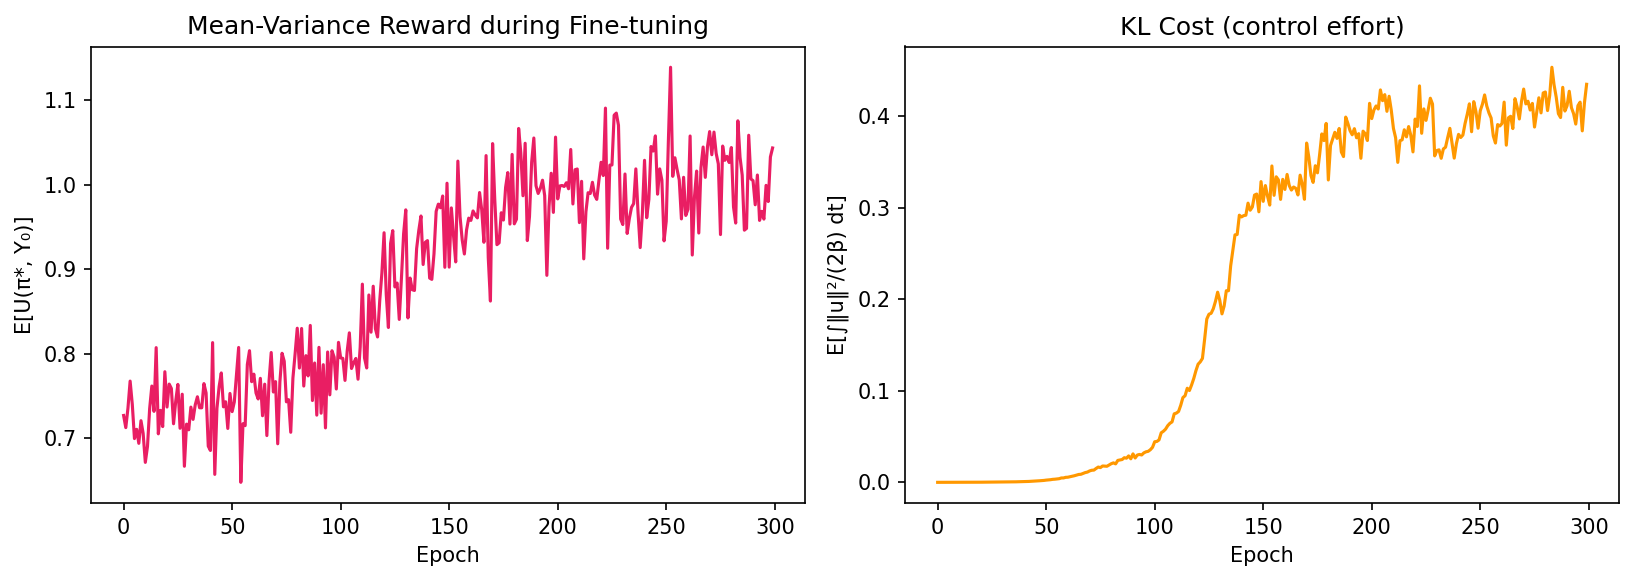
\includegraphics[width=0.75\textwidth]{figures/finetune_training.png}
  \caption{Fine-tuning training curves. Left: portfolio reward (Equation~\ref{eq:reward})
           across epochs; reward increases monotonically, confirming the control
           successfully shapes the distribution. Right: KL cost (Equation~\ref{eq:kl-girsanov})
           per epoch; the control effort stabilizes after approximately 50 epochs.}
  \label{fig:ft-curves}
\end{figure}

\end{document}
